\chapter{Manual Inspection Protocol and Evaluation Sample}
\label{appendix:manual-inspection}

This appendix documents how the inspected role sample was interpreted during the evaluation. It
supports the discussion of dataset noise, heterogeneous recruitment sources, and ambiguity
handling. The full 300-role inspection file is preserved separately as inspection\_results.json;
only the necessary protocol and summary are included here to keep the thesis appendix readable.

\section{Manual Label Definitions}
\label{appendix:manual-label-definitions}

\begin{table}[H]
    \centering
    \caption{Manual label definitions used in the evaluation}
    \label{tab:frontend-catalog-statistics}
    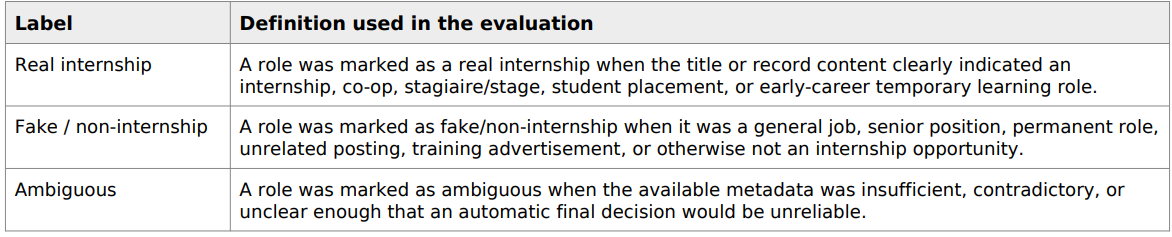
\includegraphics[width=\textwidth]{tables/appendices/Manual label definitions used in the evaluation.png}
\end{table}

\section{Human Inspection Sample Summary}
\label{appendix:human-inspection-summary}

\begin{table}[H]
    \centering
    \caption{Human inspection sample summary}
    \label{tab:frontend-catalog-statistics}
    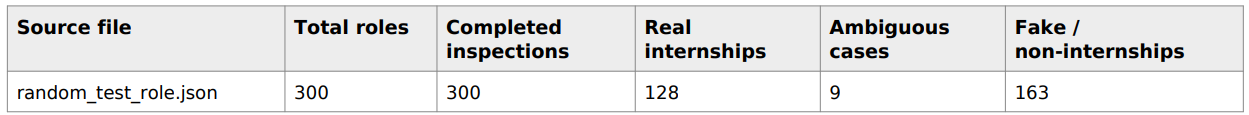
\includegraphics[width=\textwidth]{tables/appendices/Human inspection sample summary.png}
\end{table}

The manual sample confirms that scraped recruitment data contained a mixed set of valid
internships, non-internship roles, and borderline cases. This is the empirical basis for treating
internship discovery as a semantic filtering and uncertainty-management problem rather than a
simple keyword-search problem.

\section{Example Inspected Records}
\label{appendix:example-inspected-records}

\begin{table}[H]
    \centering
    \caption{Example inspected records}
    \label{tab:frontend-catalog-statistics}
    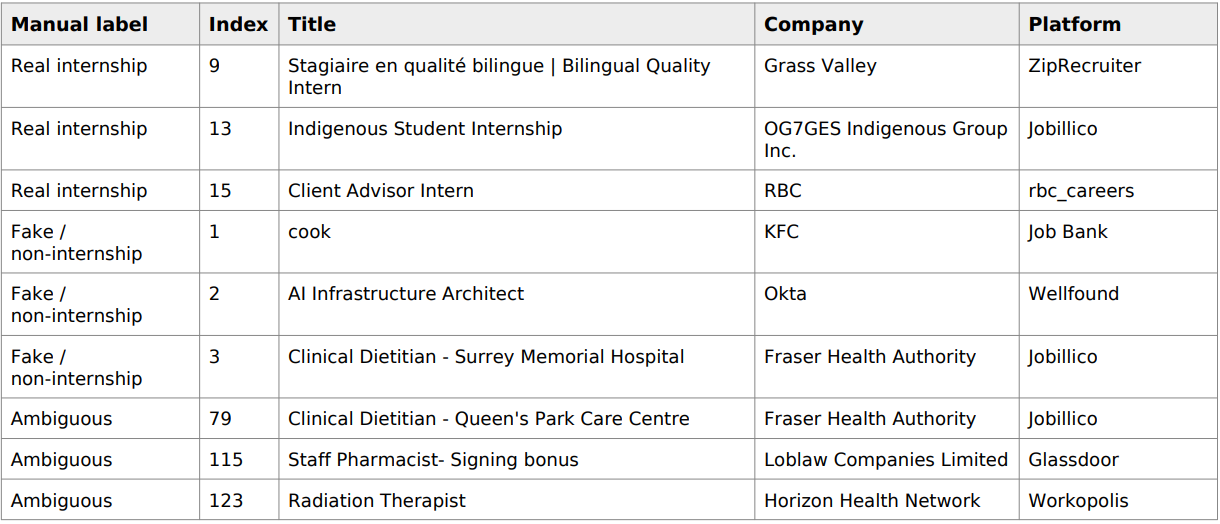
\includegraphics[width=\textwidth]{tables/appendices/Example inspected records.png}
\end{table}

\section{Files Supporting Appendix A}
\label{appendix:files-supporting-appendix-a}

\begin{table}[H]
    \centering
    \caption{Files supporting Appendix A}
    \label{tab:frontend-catalog-statistics}
    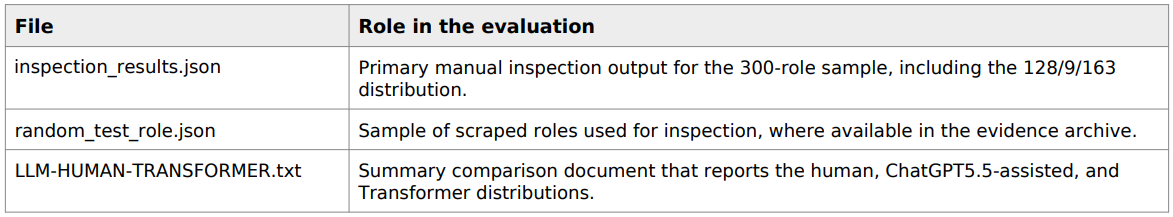
\includegraphics[width=\textwidth]{tables/appendices/Files supporting Appendix A.png}
\end{table}



\chapter{Internship Detection and Classification Evidence}
\label{appendix:classification-evidence}

This appendix supports the classification results discussed in Chapter 6. Human review is treated as
the reference for the inspected sample. ChatGPT5.5-assisted review is reported as sample-level
agreement with that reference, not as a claim of universal accuracy. The Transformer is evaluated
as a binary real/fake detector because it does not output an ambiguous class.

\section{Classification Comparison Table}
\label{appendix:classification-comparison-table}

\begin{table}[H]
    \centering
    \caption{Classification comparison table}
    \label{tab:frontend-catalog-statistics}
    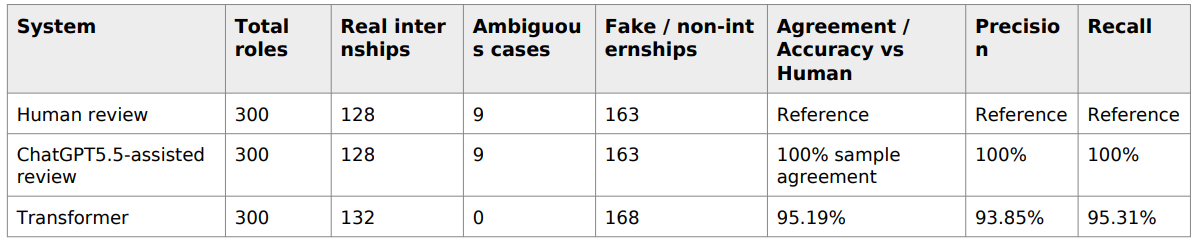
\includegraphics[width=\textwidth]{tables/appendices/Classification comparison table.png}
\end{table}

\section{Interpretation of the Metrics}
\label{appendix:interpretation-of-metrics}

Precision measures how trustworthy the system is when it classifies a role as a real internship. A
high precision score means that fewer fake or non-internship roles are incorrectly accepted as real
internships.

Recall measures how many real internships the system successfully finds. A high recall score
means that fewer genuine internships are missed.

The Transformer achieved 95.19\% accuracy, 93.85\% precision, and 95.31\% recall against the
human clear real/fake cases. Since the Transformer does not produce an ambiguous label,
ambiguous cases remain better handled through manual or ChatGPT5.5-assisted review. This
interpretation supports the uncertainty-management focus of the thesis.

\section{Classification Evidence Files}
\label{appendix:classification-evidence-files}

\begin{table}[H]
    \centering
    \caption{Classification evidence files}
    \label{tab:frontend-catalog-statistics}
    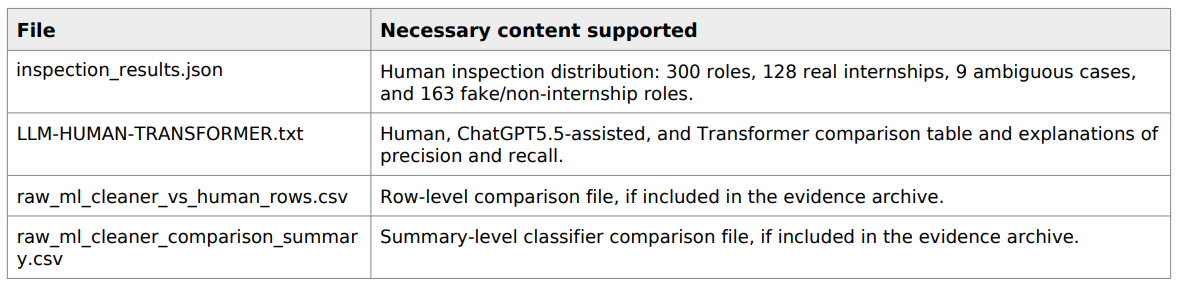
\includegraphics[width=\textwidth]{tables/appendices/Classification evidence files.png}
\end{table}

\chapter{Semantic Enrichment Rules, Vocabularies, and Pipeline Logic}
\label{appendix:semantic-enrichment-rules}

This appendix records the essential implementation logic behind the semantic enrichment pipeline
without reproducing the full codebase. It supports the claim that the pipeline combines
deterministic cleaning, rule-based internship signals, embedding-based classification, skill
extraction, domain categorization, deduplication, and manual-review indicators.

\section{Pipeline Flow}
\label{appendix:pipeline-flow}

\begin{itemize}
    \item Load raw JSON records from scraped or provided recruitment data.
    \item Normalize heterogeneous fields into a common internal representation.
    \item Remove invalid records and reduce noisy descriptions while preserving useful text structure.
    \item Deduplicate records using normalized links, title/company/location keys, and similarity checks.
    \item Apply transparent internship scoring rules using positive and negative role signals.
    \item Apply local Transformer/prototype classification when enabled and blend it with rule evidence.
    \item Extract controlled skills and classify a broad domain/category.
    \item Assign internship probability, final label, and manual-review indicators.
    \item Export accepted records into frontend-ready JSON for browsing, filtering, and inspection.
\end{itemize}

\section{Core Implementation Files}
\label{appendix:core-implementation-files}

\begin{table}[H]
    \centering
    \caption{Core implementation files}
    \label{tab:frontend-catalog-statistics}
    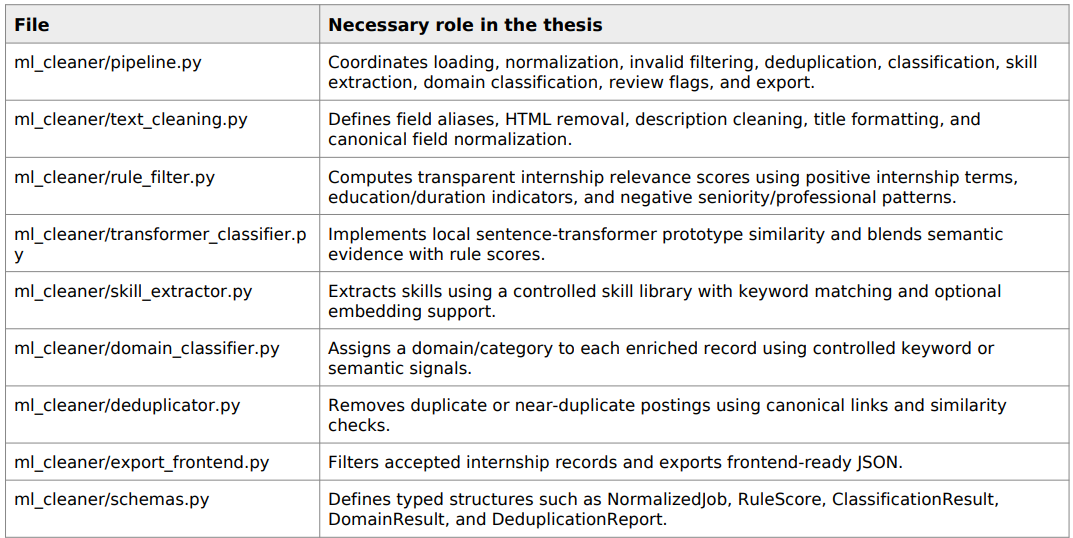
\includegraphics[width=\textwidth]{tables/appendices/Core implementation files.png}
\end{table}

\section{Configuration and Vocabulary Files}
\label{appendix:configuration-and-vocabulary-files}

\begin{table}[H]
    \centering
    \caption{Configuration and vocabulary files}
    \label{tab:frontend-catalog-statistics}
    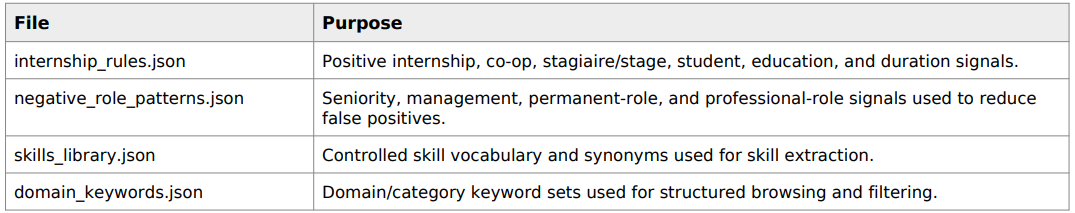
\includegraphics[width=\textwidth]{tables/appendices/Configuration and vocabulary files.png}
\end{table}

\section{Uncertainty and Manual-Review Logic}
\label{appendix:uncertainty-and-manual-review-logic}

The implementation does not force every uncertain posting into a confident final interpretation. The
manual-review indicator is triggered by uncertainty conditions such as probability falling inside a
review range, disagreement between rule and semantic evidence, weak semantic margin, or
conflict between an internship-looking title and a negative final decision. This supports RQ4 by
preserving ambiguity instead of hiding it behind a binary decision.

\begin{verbatim}
manual_review = (
    probability inside review range
    OR rule/semantic disagreement
    OR internship title conflicts with final decision
    OR semantic margin is weak
)
\end{verbatim}


\chapter{Structured Internship Schema and Frontend Catalog Evidence}
\label{appendix:structured-internship-schema}

This appendix shows the structured output expected from the enrichment pipeline and the
frontend-facing fields used for discovery. It supports RQ2 and RQ3 by connecting semantic
enrichment to concrete searchable and filterable record fields.

\section{Frontend-Ready Internship Record Schema}
\label{appendix:frontend-ready-schema}

\begin{table}[H]
    \centering
    \caption{Frontend-ready internship record schema}
    \label{tab:frontend-catalog-statistics}
    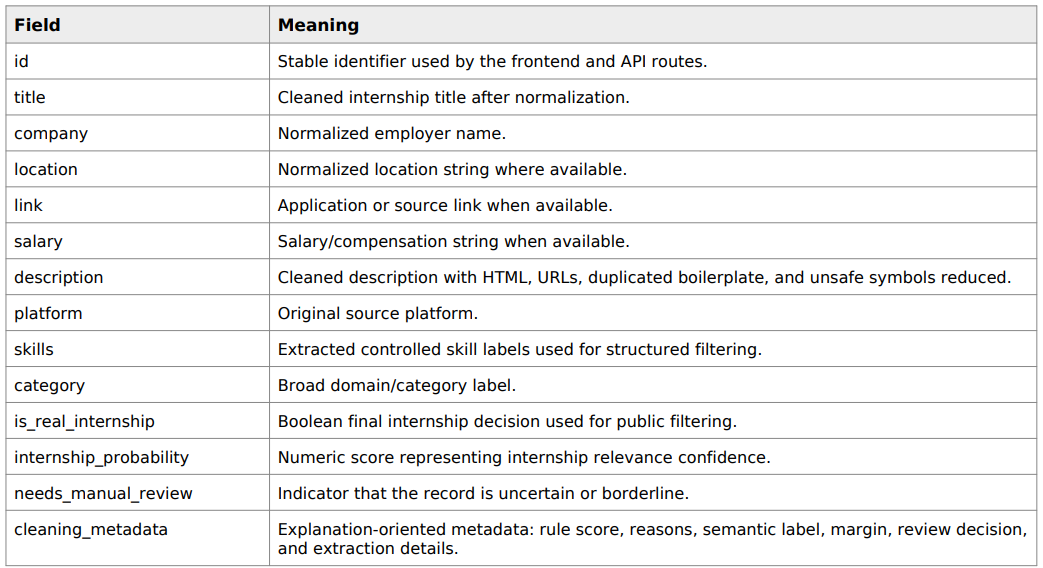
\includegraphics[width=\textwidth]{tables/appendices/Frontend-ready internship record schema.png}
\end{table}

\section{Enriched Catalog Statistics Used in Chapter 6}
\label{appendix:enriched-catalog-statistics}

\begin{table}[H]
    \centering
    \caption{Enriched catalog statistics used in Chapter 6}
    \label{tab:frontend-catalog-statistics}
    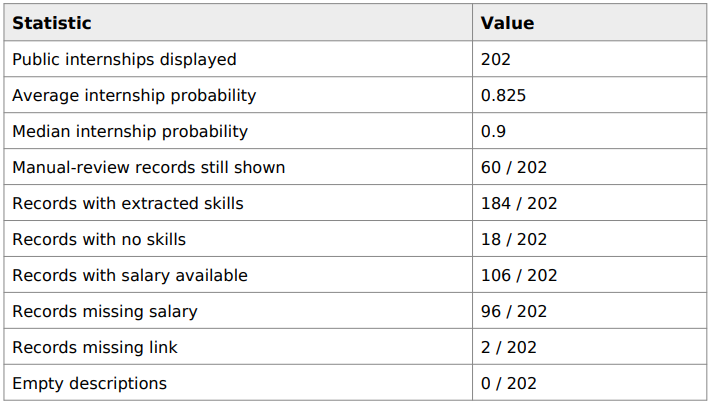
\includegraphics[width=\textwidth]{tables/appendices/Enriched catalog statistics used in Chapter 6.png}
\end{table}

\section{Example Structured Record Shape}
\label{appendix:example-structured-record-shape}

The following reduced example shows the record shape, not the full description text. It
demonstrates the fields that make the enriched catalog searchable, filterable, and reviewable.

\begin{verbatim}
{
  "id": "...",
  "title": "SAP IT Business Analyst Co-Op (Jan 2026)",
  "company": "Lockheed Martin Canada",
  "location": "Ontario",
  "skills": ["business", "education", "finance", "operations"],
  "category": "business",
  "is_real_internship": true,
  "internship_probability": 0.65,
  "needs_manual_review": true,
  "cleaning_metadata": {
    "rule_score": 0.55,
    "internship_label": "real internship",
    "semantic_label": "real internship",
    "semantic_margin": 0.0254
  }
}
\end{verbatim}

\section{Frontend Discovery Fields}
\label{appendix:frontend-discovery-fields}

Search and filtering are supported by enriched fields such as title, company, location, skills,
category, salary, description, internship probability, and review indicators. This supports structured
discovery without claiming formal user satisfaction or a completed user study.

\section{Files Supporting Appendix D}
\label{appendix:files-supporting-appendix-d}

\begin{table}[H]
    \centering
    \caption{Files supporting Appendix D}
    \label{tab:frontend-catalog-statistics}
    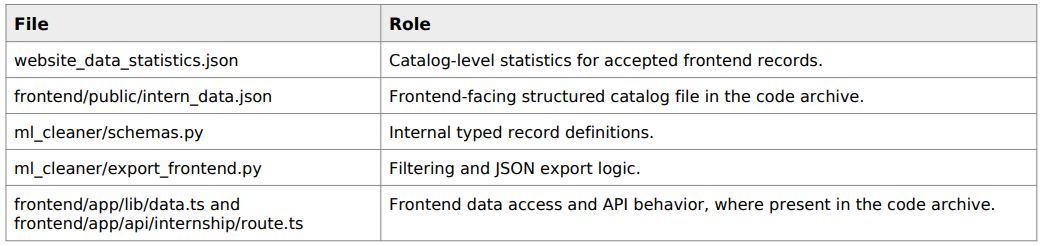
\includegraphics[width=\textwidth]{tables/appendices/Files supporting Appendix D.png}
\end{table}


\chapter{Evaluation Logs and Reproducibility Evidence}
\label{appendix:evaluation-logs-reproducibility}

This appendix lists the proof files needed to verify the operational and frontend-oriented
measurements used in Chapter 6. The logs are not pasted in full because the thesis should not
become a raw technical dump. The files should be kept in the evidence archive alongside the
thesis.

\section{Search and Filter Timing Evidence}
\label{appendix:search-filter-timing-evidence}

\begin{table}[H]
    \centering
    \caption{Search and filter timing evidence}
    \label{tab:frontend-catalog-statistics}
    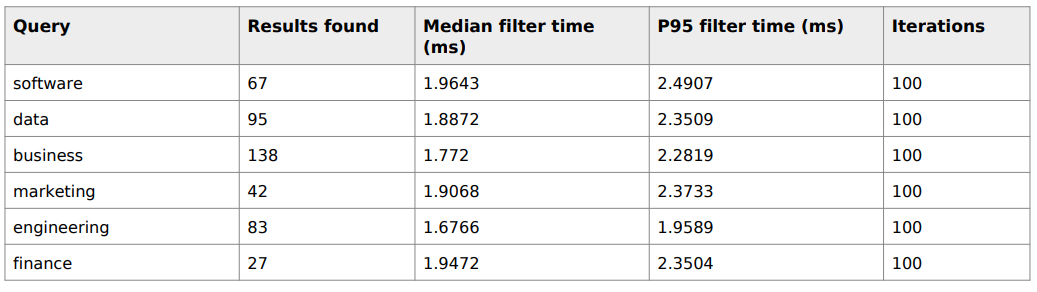
\includegraphics[width=\textwidth]{tables/appendices/Search and filter timing evidence.png}
\end{table}

\section{Local Frontend Response Evidence}
\label{appendix:local-frontend-response-evidence}

\begin{table}[H]
    \centering
    \caption{Local frontend response evidence}
    \label{tab:frontend-catalog-statistics}
    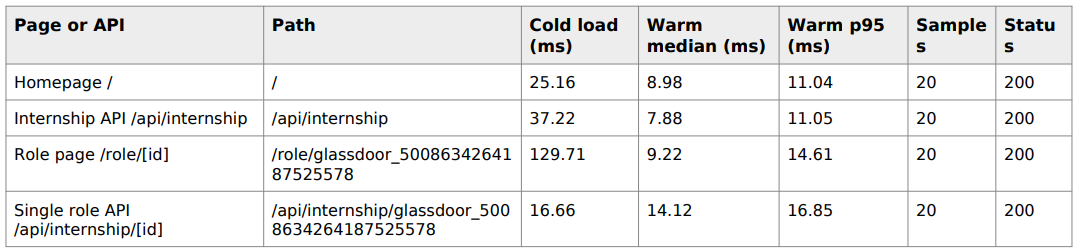
\includegraphics[width=\textwidth]{tables/appendices/Local frontend response evidence.png}
\end{table}

\section{Build and File-Size Evidence}
\label{appendix:build-and-file-size-evidence}

\begin{table}[H]
    \centering
    \caption{Build and file-size evidence}
    \label{tab:frontend-catalog-statistics}
    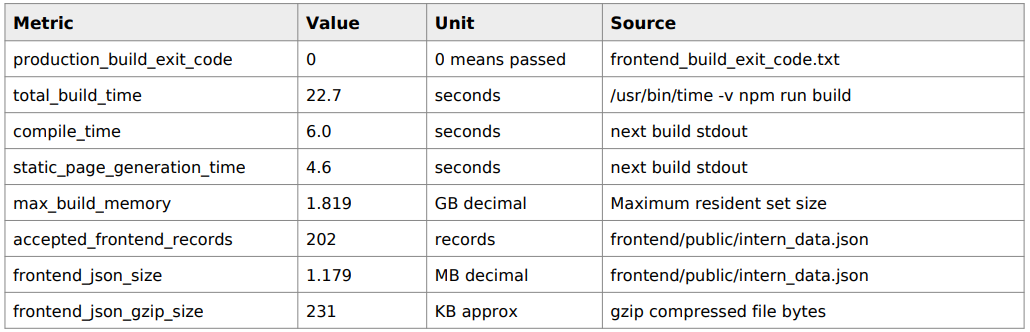
\includegraphics[width=\textwidth]{tables/appendices/Build and file-size evidence.png}
\end{table}

\section{Evidence Archive Index}
\label{appendix:evidence-archive-index}

\begin{table}[H]
    \centering
    \caption{Evidence archive index}
    \label{tab:frontend-catalog-statistics}
    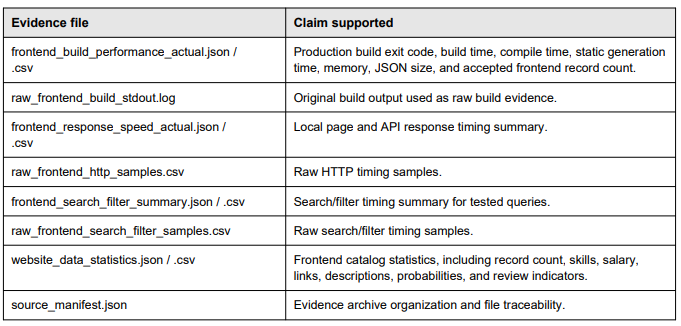
\includegraphics[width=\textwidth]{tables/appendices/Evidence archive index.png}
\end{table}

\section{Interpretation Boundary}
\label{appendix:interpretation-boundary}

These measurements should be described as local evaluation results observed under the tested
environment. They support local execution feasibility and structured discovery behavior, but they
do not prove universal cloud performance, production scalability, or user satisfaction. This
boundary is important for defending the research scope.

